\iflanguage{ngerman}
{\chapter{Einleitung}}
{\chapter{Introduction}}

\label{sec:introduction}
Electronic Health Records (EHRs) have become central to modern healthcare delivery, capturing patient trajectories through heterogeneous data streams such as demographics, diagnosis and procedure codes, medications, laboratory tests, and free-text clinical documentation. Despite their breadth, translating EHR data into actionable clinical decision support remains challenging: information is noisy, sparse, distributed over time, and encoded in formats designed primarily for documentation, billing, and storage rather than inference. These challenges motivate a large body of research on learning clinically useful representations and predictors from EHR data \cite{rajkomar2018scalable,miotto2016deeppatient}.

Clinical decision support systems (CDSS) aim to enhance medical decision-making by combining patient-specific information with clinical knowledge to generate assessments or recommendations at the point of care \cite{sutton2020cdss}. A canonical high-friction EHR workflow relevant to CDSS is diagnostic coding at discharge, where trained coders assign ICD-9-CM diagnosis codes by interpreting discharge summaries and reconciling them with structured events during the admission. This process is labor-intensive and error-prone, and inconsistency can propagate to reimbursement, epidemiological surveillance, and quality reporting. Complementary to retrospective coding, healthcare systems increasingly require prospective risk stratification: anticipating conditions likely to emerge in subsequent encounters to support follow-up planning and resource allocation.

\begin{figure}[t]
    \centering
    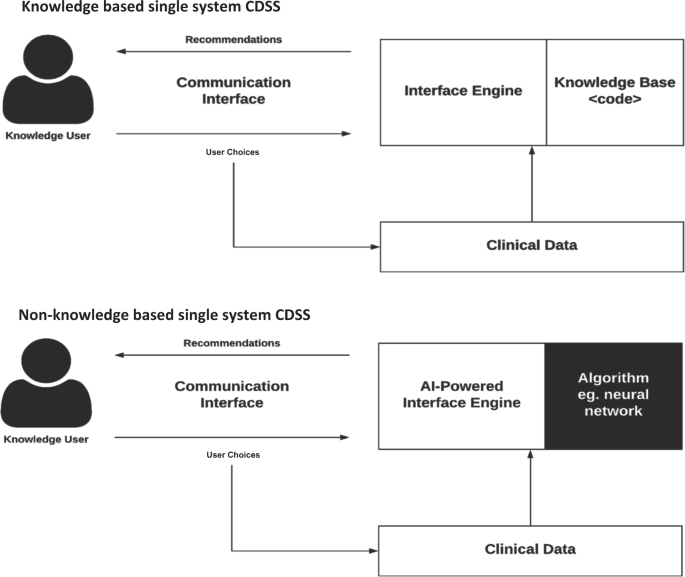
\includegraphics[width=\textwidth]{Images/CDSS.png}
    \caption{CDSS overview \cite{sutton2020cdss}}
    \label{fig:cdss-overview}
\end{figure}

Recent advances in Transformer-based large language models (LLMs) provide a promising direction for EHR-based decision support. Transformers enable flexible conditioning on long, mixed-format contexts \cite{vaswani2017attention}, while instruction tuning improves adherence to task intent and structured output formats \cite{ouyang2022training}. Parameter-efficient adaptation methods such as low-rank adaptation (LoRA) make domain and task adaptation more practical for large backbones \cite{hu2021lora}. However, diagnosis prediction presents two key tensions. First, EHR signals are inherently multimodal and sequential: structured events and narrative notes encode complementary information, and their relative utility varies between current-visit synthesis and longitudinal forecasting. Second, diagnosis prediction operates over an extremely long-tailed label space; under realistic ``top-$K$'' output budgets, improvements require better prioritisation rather than unconstrained generation.

This thesis proposes and evaluates a multimodal, sequence-generation framework for diagnosis prediction using instruction-tuned, decoder-only Transformer backbones (e.g., LLaMA-style models) \cite{touvron2023llama} adapted via parameter-efficient fine-tuning. Two complementary pipelines are studied: a direct ICD code generation baseline (\textit{CodeGen}) and a clinically aligned diagnosis-term generation pipeline (\textit{TextGen}) that maps predicted diagnosis phrases back to ICD-9 codes through semantic normalisation.

Beyond multimodal fusion, the thesis investigates whether structured biomedical knowledge can improve predictive performance and interpretability. EHR datasets may under-express clinically relevant links---risk factors, complications, and medication--indication relationships---within any single admission, particularly for rare diagnoses. To mitigate this sparsity, we construct a large UMLS-centric clinical knowledge graph (KG) \cite{bodenreider2004umls} and design a patient-conditioned retrieval mechanism that extracts short, clinically meaningful paths between patient context concepts and candidate diagnoses. These paths are linearised as concise ``medical facts'' integrated into the model context and used during KG-augmented fine-tuning, encouraging the model to treat KG evidence as privileged signal rather than distracting noise.

The empirical results obtained so far support three key messages. First, task-specific fine-tuning is essential: raw instruction-tuned models are insufficient for reliable ICD prediction without adaptation. Second, diagnosis-term generation with semantic normalisation provides a strong and consistent baseline across model sizes. Third, naive KG prompting at inference time does not reliably help; in contrast, KG-augmented fine-tuning yields more consistent gains, with the most meaningful improvements occurring in tail (rare-code) settings---consistent with the hypothesis that structured knowledge acts as an inductive bias for ranking under strict output budgets.

\paragraph{Dataset context.}
Experiments are performed on MIMIC-IV, a large, publicly available, deidentified EHR dataset sourced from Beth Israel Deaconess Medical Center and released to support clinical research \cite{johnson2023mimiciv}.

\paragraph{Thesis structure.}
Chapter~\ref{sec:background} formalises the prediction problems, input modalities, and research objectives.
Chapter~\ref{sec:related} reviews related work in multimodal EHR modelling, LLM adaptation, and knowledge-augmented clinical prediction.
Chapter~\ref{sec:methods} details cohort construction, leakage control, model architectures, KG construction, and KG integration.
Chapter~\ref{sec:results} reports experimental results for both tasks, including hierarchical and head--tail analyses.
Chapter~\ref{sec:conclusion} concludes with limitations and directions for further work.







% Electronic Health Records (EHRs) have become a central substrate for modern healthcare delivery, capturing patient trajectories through heterogeneous data streams such as demographics, diagnosis and procedure codes, medications, laboratory tests, and free-text clinical documentation. Yet, despite their breadth, translating EHR data into actionable clinical decision support remains challenging: much of the information is noisy, sparse, distributed over time, and encoded in formats designed for billing or documentation rather than inference. These limitations are especially pronounced in hospital medicine and critical care, where clinical complexity and multimorbidity are common, and where delayed or incomplete synthesis of available evidence can affect both administrative workflows and downstream care planning \cite{mimiciv}.

% A canonical example of high-friction EHR usage is diagnostic coding at discharge, where trained coders assign ICD-9-CM diagnosis codes by interpreting discharge summaries and reconciling them with structured events during the admission. This process is labor-intensive and error-prone, and inconsistent coding can propagate to reimbursement, epidemiological surveillance, and quality reporting. At the same time, hospitals increasingly require prospective risk stratification: anticipating which diagnoses are likely to appear in subsequent encounters so that follow-up, screening, and resource allocation can be planned proactively. These two needs---retrospective coding and prospective forecasting---are related instances of a broader clinical decision support objective: to summarise a patient’s evolving state and produce clinically meaningful predictions grounded in available evidence \cite{cdss_overview}.

% Recent advances in large language models (LLMs) suggest a promising modeling direction for EHR-based decision support: instruction-tuned, decoder-only Transformers can consume long, mixed-format prompts and produce structured outputs, while also providing natural-language rationales when appropriately constrained. However, directly applying LLMs to diagnosis prediction introduces two core tensions. First, EHR signals are inherently multimodal and sequential---structured events and narrative notes contribute complementary information, and the relative usefulness of each modality varies with task framing (current-visit synthesis vs.\ longitudinal forecasting). Second, diagnosis prediction operates over an extremely long-tailed label space with strict budget constraints in practical generation (e.g., emitting only a limited number of diagnoses), meaning that improved recall often requires better prioritisation rather than unconstrained output.

% This thesis proposes and evaluates a multimodal, sequence-generation framework for diagnosis prediction using instruction-tuned LLM backbones fine-tuned with parameter-efficient adaptation. Two complementary pipelines are studied: a direct ICD code generation baseline (\textit{CodeGen}) and a clinically aligned diagnosis-term generation pipeline (\textit{TextGen}) that maps predicted diagnosis phrases back to ICD-9 codes through a semantic normalisation layer.

% Beyond multimodal fusion, the thesis investigates whether structured biomedical knowledge can improve model performance and interpretability. EHR datasets may under-express clinically relevant links---risk factors, complications, medication--indication relationships---within any single admission, particularly for rare diagnoses. To mitigate this sparsity, we construct a large UMLS-centric clinical knowledge graph (KG) and design a patient-conditioned retrieval mechanism that extracts short, clinically meaningful paths between patient context concepts and candidate diagnoses. These paths are then linearised as textual ``medical facts'' that can be injected into the LLM context and, crucially, used during training so that the model learns to treat KG evidence as privileged context rather than distracting noise \cite{umls}.

% The results to date support three key messages. First, task-specific fine-tuning is essential: raw instruction-tuned models perform near zero on direct ICD generation, while fine-tuned pipelines improve substantially. Second, TextGen provides a strong and consistent baseline across backbones and evaluation regimes, outperforming CodeGen on both micro- and macro-level metrics. Third, naive KG prompting at inference time does not reliably help; in contrast, KG-augmented fine-tuning yields consistent gains, with the most meaningful improvements occurring in long-tail (rare-code) settings---aligning with the hypothesis that structured knowledge can act as an inductive bias for ranking under strict output budgets.

% \paragraph{Thesis structure.}
% Chapter~\ref{sec:background} formalises the prediction problems, input modalities, and research objectives. Chapter~\ref{sec:related} reviews related work in multimodal EHR modelling, LLM adaptation, and knowledge-augmented clinical prediction. Chapter~\ref{sec:methods} details cohort construction, leakage control, model architectures, KG construction, and KG integration. Chapter~\ref{sec:results} reports experimental results for both tasks, including hierarchical and head--tail analyses. Chapter~\ref{sec:conclusion} concludes with limitations and directions for further work.

% % Optional: overview figure placeholder
% \begin{figure}[t]
%     \centering
%     % Replace with your own re-drawn pipeline (recommended) or a schematic you create.
%     
\includegraphics[width=\linewidth]{Images/Empty.png}
%     \caption{High-level overview of the proposed multimodal diagnosis prediction framework with knowledge-graph enrichment. Structured EHR events and clinical text are serialised into prompts for LLM-based generation (CodeGen / TextGen). Patient-conditioned KG retrieval provides concise relational evidence (short paths) that is integrated into the model context, particularly during KG-augmented fine-tuning.}
%     \label{fig:overview-pipeline}
% \end{figure}